% MIT License

% Copyright (c) 2022 Chiyuru

% Permission is hereby granted, free of charge, to any person obtaining a copy of this software and associated documentation files (the "Software"), 
% to deal in the Software without restriction, including without limitation the rights
% to use, copy, modify, merge, publish, distribute, sublicense, and/or sell
% copies of the Software, and to permit persons to whom the Software is
% furnished to do so, subject to the following conditions:

% The above copyright notice and this permission notice shall be included in all copies or subsubstantial portions of the Software.

% THE SOFTWARE IS PROVIDED "AS IS", WITHOUT WARRANTY OF ANY KIND, EXPRESS OR IMPLIED, INCLUDING BUT NOT LIMITED TO THE WARRANTIES OF MERCHANTABILITY,
% FITNESS FOR A PARTICULAR PURPOSE AND NONINFRINGEMENT. IN NO EVENT SHALL THE AUTHORS OR COPYRIGHT LASTERS BE LIABLE FOR ANY CLAIM, DAMAGES OR OTHER
% LIABILITY, WHETHER IN AN ACTION OF CONTRACT, TORT OR OTHERWISE, ARISING FROM,
% OUT OF OR IN CONNECTION WITH THE SOFTWARE OR THE USE OR OTHER DEALINGS IN THE SOFTWARE.

\documentclass[UTF8]{ctexart}

\usepackage{amsmath}
\usepackage{cases}
\usepackage{cite}
\usepackage{graphicx}
\usepackage[margin=1in]{geometry}
\usepackage{float}
\geometry{a4paper}
\usepackage{fancyhdr}
\usepackage{multirow}
\usepackage{listings}
\pagestyle{fancy}
\fancyhf{}


\title{ICS-lab4实验报告}
\author{孔浩宇 PB20000113}
\date{\today}
\pagenumbering{arabic}

\begin{document}

\fancyhead[L]{孔浩宇}
\fancyhead[C]{ICS-lab4实验报告}
\fancyfoot[C]{\thepage}

\maketitle
\tableofcontents
\newpage

\section{实验目的}
    对于存储于x4000至x400F的16名学生的成绩$(0-100)$,将其升序排列并依次存储于x5000至x500F,
    并统计获得A,B成绩的学生数量,将结果依次存储在x5100与x5101中。

\section{实验原理}
    \subsection{实现if语句}
    \begin{enumerate}
        \item [(1)]if A==B.
        \begin{lstlisting}[basicstyle=\ttfamily,language={[x86masm]Assembler}]
                ADD     R, A, #0
                NOT     R, R
                ADD     R, R, #1    ; R=-A
                ADD     R, R, B     ; R=B-A
                BRnp     AFTER      ;
                ...                 ; if(B-A==0) do this
            AFTER                   
        \end{lstlisting}

        \item [(2)]if A>B.
        \begin{lstlisting}[basicstyle=\ttfamily,language={[x86masm]Assembler}]
            ADD     R, A, #0
            NOT     R, R
            ADD     R, R, #1    ; R=-A
            ADD     R, R, B     ; R=B-A
            BRzp     AFTER      ;
            ...                 ; if(B-A<0) do this
        AFTER                   
        \end{lstlisting}

        \item [(3)]if A$\geq$B.
        \begin{lstlisting}[basicstyle=\ttfamily,language={[x86masm]Assembler}]
            ADD     R, A, #0
            NOT     R, R
            ADD     R, R, #1    ; R=-A
            ADD     R, R, B     ; R=B-A
            BRp     AFTER      ;
            ...                 ; if(B-A<=0) do this
        AFTER                   
        \end{lstlisting}

        \item [(4)]其余A<B, A$\leq$B类似,不再赘述.
    \end{enumerate}

    \clearpage
    \subsection{数据交换}
    将R0 (起始)与 R0 + 1内存中的数据交换,利用R3存储读取前一个数,R4读取后一个数,
    再利用STR指令将R3的值存储到后一个地址单元,将R4的值存储到前一个地址单元。
    \begin{lstlisting}[basicstyle=\ttfamily,language={[x86masm]Assembler}]
        LDR R3, R0, #0
        ADD R0, R0, #1
        LDR R4, R0, #0
        STR R3, R0, #0
        ADD R0, R0, #-1
        STR R4, R0, #0
        ADD R0, R0, #1
    \end{lstlisting}


\section{实验步骤}
\subsection{初始化}
\begin{enumerate}
    \item [(0)]标号
    \begin{lstlisting}[basicstyle=\ttfamily,language={[x86masm]Assembler}]
        DATA	.FILL X4000
        COPY	.FILL X5000
        COUNTER	.FILL X0010
        MAX     .FILL x500F
        ASubs	.FILL X5100
        BSubs 	.FILL X5101
        ALAST	.FILL X500C
        BLAST	.FILL X5008
        A	    .FILL #85
        B	    .FILL #75
        NUM	    .FILL #15
    \end{lstlisting}

    \item [(1)]初始化其他变量
    \begin{lstlisting}[basicstyle=\ttfamily,language={[x86masm]Assembler}]
        LD R0, DATA
    	LD R1, COPY
    	LD R2, COUNTER
    \end{lstlisting}
\end{enumerate}

\clearpage
\subsection{数据搬迁}
    用$R_0$来存储原数据首地址x4000 (DATA),用$R_1$来存储排序后数据存储的首地址x5000 (COPY),
    $R_2$的值为循环次数16,采用基址加偏移的寻址方式读取内存,$R_3$作为中间搬运工,利用LDR和STR指令先将数据搬移。
    \begin{lstlisting}[basicstyle=\ttfamily,language={[x86masm]Assembler}]
        LOOP1	BRZ NEXT1
    	LDR R3, R0, #0
    	ADD R0, R0, #1
    	STR R3, R1, #0
    	ADD R1, R1, #1
    	ADD R2, R2, #-1
    	BRNZP LOOP1
    \end{lstlisting}

\subsection{冒泡排序}
现在数据已经搬移到x4000 $\sim$ x400F,开始排序。

普通的冒泡排序需要内外两层循环,外循环n-1次,内循环n-1次,因此,我们让$R_0$和$R_1$的值都为15,
读取内存时依旧采用基址加偏移的寻址方式,$R_2$存储数据存储地址x5000,$R_3$读取前一个数,
$R_4$读取后一个数,之后需要进行比较大小,将$R_3$取反加1存储在$R_5$,然后将$R_5$和$R_4$相加的结果存储在$R_5$,
通过判断$R_5$的正负来判断$R_3$和$R_4$的大小,如果R3大于R4,即R5是正数,那么就交换这两个数,
利用STR指令将R3的值存储到后一个地址单元,将R4的值存储到前一个地址单元。

\begin{lstlisting}[basicstyle=\ttfamily,language={[x86masm]Assembler}]
    NEXT1	LD R1, NUM
    LOOP2	BRZ NEXT2
            LD R0, COPY
            LD R2, NUM
    LOOP3	BRZ AGAIN
            LDR R3, R0, #0
            ADD R0, R0, #1
            LDR R4, R0, #0
            NOT R5, R3
            ADD R5, R5, #1
            ADD R5, R5, R4
            BRp RIGHT
            STR R3, R0, #0
            ADD R0, R0, #-1
            STR R4, R0, #0
            ADD R0, R0, #1
    RIGHT	ADD R2, R2, #-1
            BRNZP LOOP3
    AGAIN	ADD R1, R1, #-1
            BRNZP LOOP2
\end{lstlisting}

\subsection{成绩分类}  
读取数据采取基址加偏移的寻址方式,R0存储最大成绩的地址x500F,R1和R2清0用来存储A和B的人数,
R3存储循环次数16,R4存储每一个数据,R5作为中间载体,存储数据取反加一的值,
R6和R7存储着A和B的临界成绩85和75,同时承担存储和R5相加后的数据,用于比较成绩。
最后将R1和R2的值分别存进地址为x5100和x5101的内存单元。

\begin{lstlisting}[basicstyle=\ttfamily,language={[x86masm]Assembler}]
    NEXT2	LD  R0, MAX
    	AND R1, R1, #0
    	AND R2, R2, #0
    	LD  R3, COUNTER
    LOOP4	BRZ FINISH
            LDR R4, R0, #0
            LD  R6, A
            LD  R7, B
            NOT R4, R4
            ADD R4, R4, #1
            ADD R6, R6, R4
            BRP BB
            NOT R5, R0
            ADD R5, R5, #1
            LD  R6, ALAST
            ADD R6, R6, R5
            BRP BB
            ADD R1, R1, #1
            BRNZP TAIL
    BB	    ADD R7, R7, R4
            BRP TAIL
            LD  R7, BLAST
            ADD R7, R7,R5
            BRP TAIL
            ADD R2, R2, #1
    TAIL	ADD R0, R0, #-1
            ADD R3, R3, #-1
            BRNZP LOOP4
\end{lstlisting}

\subsection{结束}  
\begin{lstlisting}[basicstyle=\ttfamily,language={[x86masm]Assembler}]
    FINISH	STI R1, ASubs
            STI R2, BSubs
            HALT
\end{lstlisting}

\clearpage
\subsection{代码}    
\begin{lstlisting}[basicstyle=\ttfamily,language={[x86masm]Assembler}]
	.ORIG X3000
    	LD R0, DATA
    	LD R1, COPY
    	LD R2, COUNTER
LOOP1	BRZ NEXT1
    	LDR R3, R0, #0
    	ADD R0, R0, #1
    	STR R3, R1, #0
    	ADD R1, R1, #1
    	ADD R2, R2, #-1
    	BRNZP LOOP1
NEXT1	LD R1, NUM
LOOP2	BRZ NEXT2
    	LD R0, COPY
    	LD R2, NUM
LOOP3	BRZ AGAIN
    	LDR R3, R0, #0
    	ADD R0, R0, #1
    	LDR R4, R0, #0
    	NOT R5, R3
     	ADD R5, R5, #1
    	ADD R5, R5, R4
    	BRp RIGHT
    	STR R3, R0, #0
    	ADD R0, R0, #-1
    	STR R4, R0, #0
    	ADD R0, R0, #1
RIGHT	ADD R2, R2, #-1
	    BRNZP LOOP3
AGAIN	ADD R1, R1, #-1
	    BRNZP LOOP2
NEXT2	LD  R0, MAX
    	AND R1, R1, #0
    	AND R2, R2, #0
    	LD  R3, COUNTER
LOOP4	BRZ FINISH
    	LDR R4, R0, #0
    	LD  R6, A
    	LD  R7, B
    	NOT R4, R4
     	ADD R4, R4, #1
    	ADD R6, R6, R4
    	BRP BB
    	NOT R5, R0
    	ADD R5, R5, #1
    	LD  R6, ALAST
    	ADD R6, R6, R5
    	BRP BB
    	ADD R1, R1, #1
    	BRNZP TAIL
BB	    ADD R7, R7, R4
    	BRP TAIL
    	LD  R7, BLAST
    	ADD R7, R7,R5
    	BRP TAIL
    	ADD R2, R2, #1
TAIL	ADD R0, R0, #-1
    	ADD R3, R3, #-1
    	BRNZP LOOP4

FINISH	STI R1, ASubs
    	STI R2, BSubs
    	HALT
DATA	.FILL X4000
COPY	.FILL X5000
COUNTER	.FILL X0010
MAX     .FILL x500F
ASubs	.FILL X5100
BSubs 	.FILL X5101
ALAST	.FILL X500C
BLAST	.FILL X5008
A	    .FILL #85
B	    .FILL #75
NUM	    .FILL #15
	.END
\end{lstlisting}

\clearpage
\section{实验结果}
    \begin{figure*}[htbp]
        \centering
        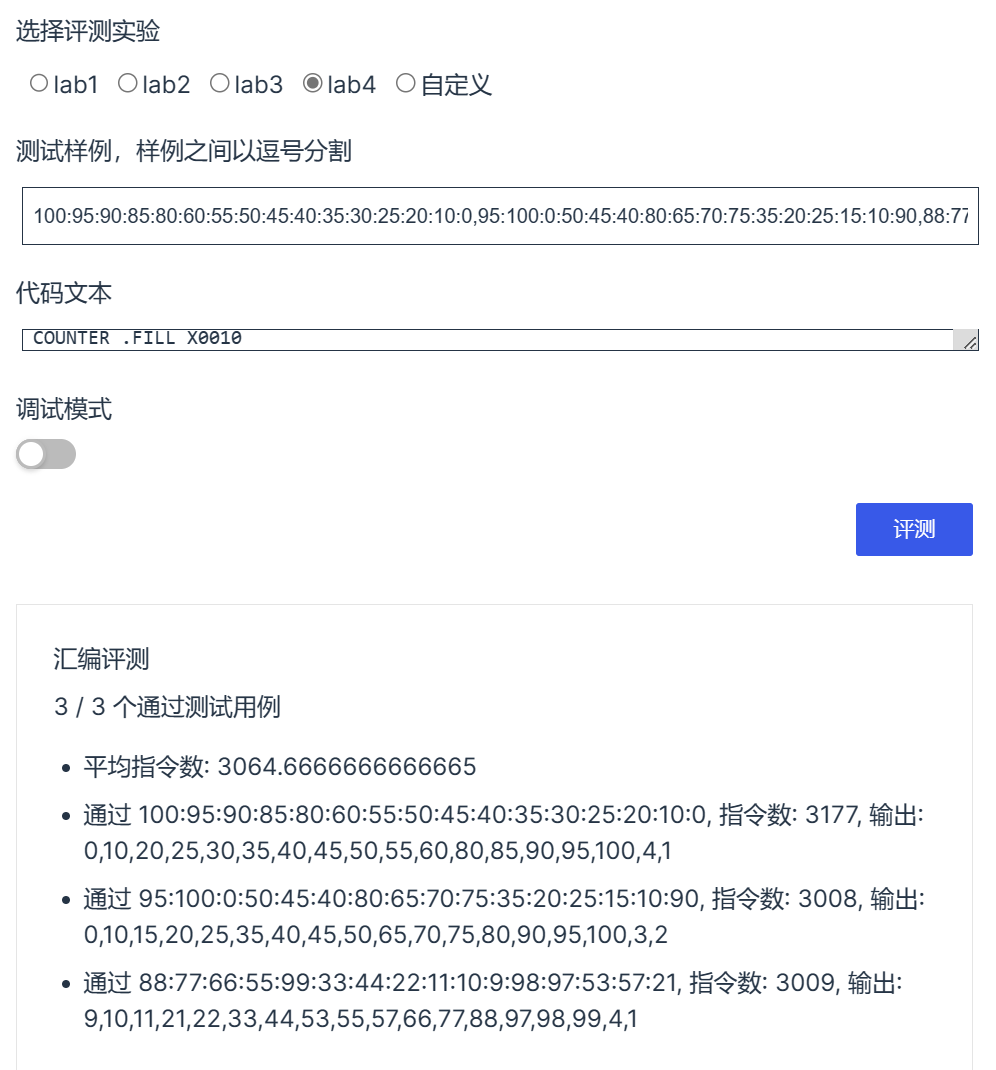
\includegraphics[scale=0.8]{r.png}
    \end{figure*}
\end{document}
\begin{lstlisting}[basicstyle=\ttfamily,language={[x86masm]Assembler}]

\end{lstlisting}